%%% ДАННЫЙ ФАЙЛ ПРЕДСТАВЛЯЕТ ПРИМЕР ИСПОЛЬЗОВАНИЯ ПАКЕТА pazh2col-win
%%% ДЛЯ ФОРМАТИРОВАНИЯ СТАТЬИ В СТИЛЕ "ПИСЕМ В АСТРОНОМИЧЕСКИЙ ЖУРНАЛ"
%%% С ИСПОЛЬЗОВАНЕМ КОДИРОВКИ WINDOWS-1251.
%%% Автор: Александр Потехин, ФТИ им. А.Ф. Иоффе, 2023 <palex@astro.ioffe.ru>.
%%% ПРЕДОСТАВЛЯЕТСЯ ДЛЯ СВОБОДНОГО ИСПОЛЬЗОВАНИЯ: Creative Commons Zero (СС0).
%%% ПОЖАЛУЙСТА, СООБЩАЙТЕ ОБ ОБНАРУЖЕННЫХ ОШИБКАХ И ПРОБЛЕМАХ ПО ВЫШЕУКАЗАННОМУ АДРЕСУ!

\documentclass{pazh2col-win}

%%% Далее можно подгрузить дополнительные пакеты.
%%% Например, пакет graphicx используется для вставки в текст рисунков:
\usepackage{graphicx}
\usepackage{amsbsy}
\usepackage{amssymb} 
\usepackage[T2A]{fontenc}
\usepackage[cp1251]{inputenc}
\usepackage[english,russian]{babel}
\usepackage{epstopdf}
\usepackage[autostyle]{csquotes}

\usepackage{cuted}   
\usepackage{lipsum}  

\usepackage[intoc,nocfg,russian]{nomencl}
\newcommand{\nomencl}[2]{#1 --- #2\nomenclature{#1}{#2}}
\setlength{\nomlabelwidth}{3em}
\setlength{\nomitemsep}{-\parsep}
\setcounter{tocdepth}{2}
\renewcommand{\nomlabel}[1]{#1 ---}
\makenomenclature

\usepackage{wrapfig}
\let\vec=\mathbf
%\graphicspath{{fig/}}
\def\mprp{\mbox{\tiny $\bot$}}
\def\mprl{\mbox{\tiny $\|$}}
\def\th{\mbox{th}}

\def\D{\mathrm{d}}
\def\beq{\begin{eqnarray}}
\def\eeq{\end{eqnarray}}
\def\ee{\varepsilon}
\def\lm{\lambda}
\newcommand{\prp}[1]{#1_{\mbox{\tiny $\bot$}}}
\newcommand{\pprl}[1]{#1_{\mbox{\tiny $\|$}}}
\newcommand{\ii}{\mathrm{i}} % мнимая единица
\newcommand{\dd}{\mathrm{d}} % дифференциал
\newcommand{\eee}{\mathrm{e}} % основание натуральных логарифмов
\def\HH{H\!\!\left(\frac{4 m^2}{\pprl{q}^2}\right)}
\def\HHi{H\!\!\left(\frac{4 m^2}{\pprl{q'^2}}\right)}
\def\HHii{H\!\!\left(\frac{4 m^2}{\pprl{q''^2}}\right)}
\def\ggg{\gamma \rightarrow \gamma \gamma}
\def\ff{\Lambda}
\def\tff{\widetilde \Lambda}
\def\1{1 \to 1 \, 2}
\def\2{1 \to 2 \, 2}
\def\S{S}
\def\J{{\cal J}}
\def\A{{\cal A}}
\def\P{{\cal P}}
\def\M{{\cal M}}
\newcommand{\bs}{\boldsymbol}

\begin{document}

%%% Список авторов задается командой \authors.
%%% В квадратных скобках размещается краткий список для верхнего колонтитула на четных страницах:
%%% ФАМИЛИЯ (заглавными буквами) - если автор только один;
%%% ФАМИЛИЯ1, ФАМИЛИЯ2 - если авторов двое;
%%% ФАМИЛИЯ1 и др. - если число авторов больше двух.
%%% В фигурных скобках размещается полный список авторов,
%%% причем каждый следующий добавляется командой \nextauth, имеющей два обязательных аргумента:
%%% в первых фигурных скобках указываются инициалы и фамилия, а во вторых - номера, соответствующие аффилиациям.
%%% Дополнительно, для основного соавтора в квадратных скобках перед фигурными указывается электронный адрес.

\authors[ШЛЕНЕВ и др.]{
  \nextauth[allen\_caleb@rambler.ru]{Д. М. Шленев}{1},
  \nextauth{Д. А. Румянцев}{2},
  \nextauth{А. А. Ярков}{2}
}

%%% Полный и краткий заголовки статьи задаются командой \titles.
%%% В квадратных скобках размещается краткий заголовок для верхнего колонтитула на нечетных страницах
%%% (для корректной печати этого колонтитула команда \titles должна располагаться после команды \authors).
%%% В фигурных скобках дается полное название.

\titles[Перенос излучения]{Перенос излучения в равновесной электронной плазме с учетом резонансного комптоновского процесса}

%%% Список аффилиаций задается командой \affiliations, внутри которой каждая следующая аффилиация задается командой \nextaffil. 
%%% При этом последовательная нумерация аффилиаций производится автоматически.
%%% Однако, авторы должны сами проконтролировать соответствие этому списку номеров, указанных в командах \nextauth выше.

\affiliations{
\nextaffil{Ярославское высшее военное училище противовоздушной обороны имени Маршала Советского Союза Л.А. Говорова, Ярославль, Россия}
\nextaffil{Ярославский государственный университет им. П.Г. Демидова, Ярославль, Россия}
}

%%% Следующая команда задает содержание строк, в которых указываются ключевые даты:
\def\postupila{Поступила в редакцию ??.??.2026~г.
 \\
После доработки ??.??.20??~г.; принята к публикации ??.??.20??~г.}

%%% Следующая команда задает содержание нижнего колонтитула:
\def\journame{ПИСЬМА В АСТРОНОМИЧЕСКИЙ ЖУРНАЛ ~ том ?? ~ \textnumero~?? ~ 20??}

%%% Аннотация задается как аргумент команды \wideabstract. 
%%% В конце аннотации, внутри этой команды, задаются ключевые слова как аргумент команды \keywords.
%%% После них можно вставить "\doi{}", чтобы зарезервировать место для DOI.

\wideabstract{Получено аналитическое решение кинетического уравнения для нахождения функции распределения фотонов двух возможных поляризаций в равновесной нерелятивистской электронной плазме и относительно слабом магнитном поле $B\lesssim 10^{13}$ Гс за счет процесса комптоновского рассеяния и с учетом резонанса на виртуальном электроне. С помощью преобразования Лапласа и разложения функции распределения по полиномам Лежандра задача сведена к системе дифференциальных уравнений. Проведено сравнение аналитической модели спектра излучения фотонов с результатами, полученными методом Монте-Карло. Показано, что предложенная модель достаточно хорошо описывают вклад резонансного эффекта Комптона в формирование спектра излучения в области циклотронных линий.
\keywords{нейтронные звезды, магнитное поле, уравнение Компанейца.}
% Заготовка для номера DOI (можно вставить, когда он будет известен):
\doi{10.31857/S...}
} 

%=========================================================

\section{Введение}
\label{introduction}

Спектральные особенности излучения, сопровождающего аккрецию с большого горячего объекта на нейтронную звезду в тесной двойной системе, представляют собой важный источник информации о строении нейтронных звезд, поэтому их объяснение является актуальной задачей.


Существует несколько основных способов решения задачи переноса излучения. Один из~них заключается в решении системы интегро-дифференциальных уравнений, соответствующих системе уравнений Больцмана, составляемых для каждой компоненты среды. Этот метод разрабатывался в работе (Месарош и Нагель, 1985), цикле статей (Беккер и Вольф, 2007, Беккер и др., 2012, Беккер и Вольф, 2022), а также цикле работ (Нисимура, 2003, 2005, 2008, 2011). С другой стороны, для численного анализа переноса излучения с учетом резонансного комптоновского процесса в последнее время активно используется метод Монте-Карло. Одними из первых его применяли Арайя и Хардинг, 1999, 2000, далее он совершенствовался в работах (Шенгерр и др., 2007), цикле работ (Муштуков и др., 2021, 2022, Муштуков и Портегис Цварт, 2023). Метод Монте-Карло является достаточно мощным инструментом для моделирования сложных физических систем, но имеет существенный недостаток в виде медленной сходимости результата. Однако аналитическое решение подобной задачи, по-видимому, в литературе отсутствует. В данной работе приводится аналитическое решение задачи переноса излучения в равновесной нерелятивистской электронной плазме при относительно слабом магнитном поле по сравнению с критическим: $B\lesssim B_e = m^2/e = 4.41 \times 10^{13}$ Гс\footnote{В данной работе используется естественная система единиц: $c = \hbar = k_{\rm{B}} = 1$, $m$ -- масса электрона, $e > 0$ -- элементарный заряд.}, с учетом резонанса в комптоновском процессе.

%%%%%%%%%%%%%%%%%%%%%%%%%%%%%%%%%%%%%%%%%%%%%%%%%

\section{Решение кинетического уравнения}
\label{section_A}

Для решения кинетического уравнения рассмотрим достаточно малую область аккреционной колонки с цилиндрической геометрией. Ось $z$ вдоль магнитного поля  направлена по оси цилиндра. Размеры области будем считать таковыми, что внутри нее можно считать индукцию магнитного поля, температуру и концентрацию среды постоянными. Вещество внутри будем рассматривать как равновесную зарядово-симметричную плазму, состоящую из электронов и ионов, которая, в нашей модели, вморожена в магнитное поле. Будем считать плазму нерелятивистской, $eB \gg T^2$ с химическим потенциалом $\mu = 0$ (см., например, работу Шенгерра 2007). В этом случае электроны будут в основном занимать основной уровень Ландау. У основания этой области поместим стационарный изотропный источник фотонов, которые далее распространяются в плазме. При этом мы не учитываем взаимодействие фотонов с ионами, поскольку из-за их высокой массы сечение рассеяния на них мало по сравнению с рассеянием на электронах при энергиях фотонов, намного превосходящих энергию ионного циклотронного резонанса. Кроме того, будем полагать, что колонка достаточно тонкая, что изменением функции распределения в поперечном по отношению к магнитному полю направлению можно пренебречь.

С другой стороны, при взаимодействии фотонов с электронами плазмы необходимо учитывать две составляющие влияния активной среды на протекающие в ней квантовые процессы. Первая: это модификация амплитуд процессов, что приводит к возможности появления резонансов, например, в комптоновском процессе. Вторая: модифицируются поляризационные и дисперсионные свойства частиц, вследствие чего могут открываться каналы реакций, которые запрещены или сильно подавлены в вакууме, такие как поглощение и рождение фотона электроном.

С точки зрения поляризационных свойств в замагниченной плазме фотон имеет эллиптические поляризации и три возможных поляризационных состояния. Но в присутствии зарядово-симметричной, $\mu = 0$, т.н. поледоминирующей среды ($eB\gg T^2$) векторы поляризации будут такими же, как в магнитном поле без плазмы (Чистяков и др., 2012, Румянцев и др., 2026а):
%
\begin{equation}
\label{eps}
\varepsilon^{(1)}_\mu=\frac{(q\varphi )_\mu}{\sqrt{q\varphi\varphi q}} ,\quad
\varepsilon^{(2)}_\mu=\frac{(q\tilde{\varphi})_\mu}{\sqrt{q\tilde{\varphi}\tilde{\varphi} q}}\, ,
\end{equation}
 где $\varphi_{\mu \nu} =  F_{\mu \nu} /B$ -- обезразмеренный тензор электромагнитного поля и ${\tilde \varphi}_{\mu \nu} = \varepsilon_{\mu \nu \rho \sigma} \varphi_{\rho \sigma}/2$ -- тензор, дуальный к нему,  $q^\mu = (\omega, \vec{q})$ -- 4-вектор энергии-импульса фотона, а также введены обозначения $q_{\mprl}^2 = \omega^2 - q_z^2$ и $q_{\mprp}^2 = q_x^2 + q_y^2$. Компоненты третьего вектора поляризации оказываются обратно пропорциональны индукции магнитного поля и могут быть устранены калибровочным преобразованием. Здесь индексы 1 и 2 соответствуют $X-$ и $O-$модам, которые обычно используются в литературе (см., например, монографию Гинзбурга, 1967). Вывод о совпадении векторов поляризации в зарядово-симмметричной поледоминирующей плазме с векторами поляризации в магнитном поле без плазмы с точностью до слагаемых порядка $O(1/B^2)$ и $O(\alpha^2)$, где $\alpha$ -- постоянная тонкой структуры, находится в согласии с результатами Шабада, 1988 и -- после соответствующих преобразований (выбора пространственной части вектора $\varepsilon^{(2)}$ и перехода в систему координат, в которой вектор импульса фотона направлен вдоль оси $z$) -- Потехина и др., 2004.

Таким образом, для рассеяния фотона на электроне кинематически разрешены четыре парциальных канала: $e\gamma^{(1)}\to e\gamma^{(1)}$, $e\gamma^{(2)}\to e\gamma^{(2)}$, $e\gamma^{(2)}\to e\gamma^{(1)}$, $e\gamma^{(1)}\to e\gamma^{(2)}$.

Исходя из свойств аккреционной колонки, которые обсуждались выше, стационарное уравнение Больцмана для нахождения функции распределения фотона в поляризационном состоянии $\lambda=1,2$ можно записать следующим образом:
%
\begin{eqnarray}
\label{Kineq:Gen}
\nonumber
&&x\frac{\partial f^{(\lambda)}_\omega(z,x)}{\partial z}=\sum\limits_{\lambda'=1}^{2} 
\int \dd W_{_{e\gamma^{(\lambda)} \to e\gamma^{(\lambda')} }} \times
\\
\nonumber
&&\times\{f_{E'}(1-f_E)f^{(\lambda')}_{\omega'}(z, x') (1+f_\omega^{(\lambda)}(z, x))-
\\
&&-f_E (1-f_{E'}) f_\omega^{(\lambda)}(z,x)(1+f_{\omega'}^{(\lambda')}(z, x'))\}\, .
\end{eqnarray}
%
Здесь введены обозначения: \scalebox{1}[1.0]{ $x=\cos\theta$, $x'=\cos\theta'$}, где $\theta$, $\theta'$ -- углы между магнитным полем и импульсами начального и конечного фотона соответственно, $f_\omega^{(\lambda)}, f_{\omega'}^{(\lambda')}$ -- неравновесные функции распределения начальных и конечных фотонов, которые подлежат определению,\linebreak $f_E=(\exp[E/T]+1)^{-1}, f_{E'}=(\exp[E'/T]+1)^{-1}$ \linebreak -- равновесные функции распределения начальных и конечных электронов с энергиями $E$ и $E'$ при нулевом химическом потенциале. \linebreak $\dd W_{_{e\gamma^{(\lambda)} \to e\gamma^{(\lambda')} }}$ --  дифференциальный коэффициент поглощения фотона, определяющий вероятность комптоновского рассеяния.

Пользуясь методикой, разработанной в работах (Компанеец, 1956) и (Любарский, 1988), разложим уравнение~(\ref{Kineq:Gen}) по малому изменению энергии фотона в комптоновском рассеянии \linebreak $\Delta\omega=\omega-\omega'\ll\omega$, где
%
\begin{eqnarray}
\nonumber
&&\omega' = \frac{1}{1-x'^2}\bigg(m+\omega(1-x x') -
\\
&&- \sqrt{(m+\omega(1-x x'))^2 - 2eB (1-x'^2)}\bigg)\, .
\end{eqnarray}
%
Пренебрегая индуцированным излучением, получим следующее линейное интегро-дифференциальное уравнение (Ярков и Румянцев, 2023):
%
\begin{eqnarray}
\label{eq:KinSerDeltaw}
\nonumber
&&\frac{\partial f^{(\lambda)}_\omega(z,x)}{\partial z} = \frac{1}{x} \sum_{\lambda'=1}^{2} \int_{-1}^{1}\dd x'\varphi_\omega^{\lambda\lambda'}(x,x') \times
\\
\nonumber
&&\times\bigg(f_\omega^{(\lambda')}(z,x')-f_\omega^{(\lambda)}(z,x)-
\\
\nonumber
&&- \frac{\Delta \omega}{T}\left[T \frac{\partial f_\omega^{(\lambda')}(z,x')}{\partial \omega} + f_\omega^{(\lambda')}(z,x')\right]+
\\
\nonumber
&&+ \frac{1}{2}\frac{(\Delta \omega)^2}{T^2}\bigg[T^2 \frac{\partial^2 f_\omega^{(\lambda')}(z,x')}{\partial \omega^2} + 
\\
&&+2T \frac{\partial f_\omega^{(\lambda')}(z,x')}{\partial \omega} +  f_\omega^{(\lambda')}(z,x')\bigg]\bigg)\, .
\end{eqnarray}
%
Введенная здесь функция $\varphi_\omega^{\lambda\lambda'}(x,x')$ соответствует частично проинтегрированному дифференциальному коэффициенту поглощения фотона (см., например, Ярков и Румянцев, 2023). Для первого уровня Ландау в случае узкого резонансного пика (Румянцев и др., 2026б) она может быть представлена в виде, факторизованном амплитудами подпроцессов поглощения фотона электроном, ${\cal M}^{\xi''\xi}_{e_0\gamma^{(\lambda)}\to e_1 }$, и рождения фотона электроном, ${\cal M}^{\xi'\xi''}_{e_1\to e_0\gamma^{(\lambda')}}$:
%
\begin{eqnarray}
\label{phi}
\nonumber
&&\varphi^{\lambda\lambda'}_\omega(x,x') =  \sum_{\xi,\xi',\xi''=\pm 1}
\frac{n_e \omega'}{32 \pi m \omega} \times
\\
\nonumber
\times
&&\frac{\left|{\cal M}^{\xi'\xi''}_{e_1\to e_0\gamma^{(\lambda')}}\right|^2
\left|{\cal M}^{\xi''\xi}_{e_0\gamma^{(\lambda)}\to e_1 }\right|^2}
{[\omega^2(1-x^2)+2\omega m - 2eB]^2 + (\Gamma_1^{\xi''}E_1''/2)^2} 
\times
\\
&&\times
\frac{1}{\sqrt{(m+\omega - \omega x x')^2 - x'^2 2eB}} ,
\end{eqnarray}
%
где суммирование проводится по возможным поляризационным состояниям электрона $\xi, \xi', \xi''$, \linebreak $n_e$ -- концентрация электронов в замагниченной плазме, $E''_1 = \sqrt{(p_z+q_z)^2 + M_1^2}$ -- энергия виртуального электрона, $M_1=\sqrt{m^2+2 eB}$, \linebreak $\Gamma_1^{\xi''}$ -- полная ширина поглощения электрона для магнитного поля без плазмы (Латал, 1986):
%
\begin{eqnarray}
\label{Gamma}
\nonumber
&&E_1''\Gamma_1^{\pm} \simeq \frac{e^2 (eB)^2}{\pi M_1}\frac{1}{M_1\pm m} \times
\\
&&\times\int_{0}^{\zeta}\dd x\, \eee^{-x} \frac{1-\zeta x}{\sqrt{x^2-\zeta x+1}}\, .
\end{eqnarray}
%
Здесь $\zeta=(M_1^2+m^2)/eB=2+2B_e/B$.

Преобразуя уравнение~(\ref{eq:KinSerDeltaw}) для начальных условий, соответствующих стационарному изотропному источнику фотонов: $f^{(\lambda)}_\omega(0,x)=f_{0\omega}$, получим:
%
\begin{eqnarray}
\label{FormSol}
\nonumber
&&f_\omega^{(\lambda)}(z,x)=f_{0\omega} \eee^{-{\cal \chi}_\omega^{(\lambda)}(x)\, z} +
\\
\nonumber
&&+ \frac{1}{x}\int_{0}^{z}\dd z'\int_{-1}^{1}\dd x' e^{-{\cal \chi}_\omega^{(\lambda)}(x)\, (z-z')}\,\times
\\
\nonumber
&&\times \sum_{\lambda'=1}^2\varphi_\omega^{\lambda 	\lambda'}(x,x')\bigg(f_\omega^{(\lambda')}(z,x')- 
\\
\nonumber
&&-\frac{\Delta \omega}{T} \left[	T \frac{\partial f_\omega^{(\lambda')}(z,x')}{\partial \omega} + f_\omega^{(\lambda')}(z,x') \right]+
\\
\nonumber
&&+ \frac{1}{2}\frac{(\Delta \omega)^2}{T^2}\left[	T^2 \frac{\partial^2 f_\omega^{(\lambda')}(z,x')}{\partial \omega^2} + \right.
\\
&&+\left. 2T \frac{\partial f_\omega^{(\lambda')}(z,x')}{\partial \omega}+f_\omega^{(\lambda')}(z,x')\right]\bigg)\, .
\end{eqnarray}
%

Здесь
\begin{eqnarray}
\label{chi}
{\cal \chi}_\omega^{(\lambda)}(x) = \frac{1}{x} \int_{-1}^{1} \dd x' \left\{\varphi^{\lambda 1}_\omega(x,x')+\varphi^{\lambda 2}_\omega(x,x')\right\}\, .
\end{eqnarray}
%

Используя разложение функции распределения по полиномам Лежандра и выполняя преобразование Лапласа по переменной $z$:
%
\begin{equation}
f_\omega^{(\lambda)}(z,x) = \sum_{\ell=0}^{\infty} A_\ell^{(\lambda)}(z,\omega) {\cal P}_\ell(x)\, ,
\end{equation}
%
получаем систему зацепляющихся дифференциальных уравнений на коэффициенты разложения:
\begin{eqnarray}
\label{eq:SysEqALap}
\nonumber
&&\frac{2}{2 \ell +1} \overline{A}_\ell^{(\lambda)}(s,\omega) = \int_{-1}^{1} \dd x\frac{f_{0\omega}^{(\lambda)} {\cal P}_\ell(x)}{s+{\cal \chi}^{(\lambda)}_\omega(x)}+
\\
\nonumber
&&+ \sum_{\lambda'=1}^{2}\sum_{\ell'=0}^{\infty}\frac{1}{x}\int_{-1}^{1}\dd x'\int_{-1}^{1}\dd x \frac{{\cal P}_\ell(x) {\cal P}_{\ell'}(x')}{s+{\cal \chi}_\omega^{(\lambda)}(x)} \times
\\
\nonumber
&&\times\varphi_\omega^{\lambda\lambda'}(x,x') \bigg(\overline{A}_{\ell'}^{(\lambda')}(s,\omega) -
\\
\nonumber
&&- \frac{\Delta \omega}{T}
\left[T \frac{\partial \overline{A}_{\ell'}^{(\lambda')}(s,\omega)}{\partial \omega} + \overline{A}_{\ell'}^{(\lambda')}(s,\omega)\right]+
\\
\nonumber
&&+ \frac{1}{2}\frac{(\Delta \omega)^2}{T^2}\left[	T^2 \frac{\partial^2 \overline{A}_{\ell'}^{(\lambda')}(s,\omega)}{\partial \omega^2} + \right.
\\
&&+\left. 2T \frac{\partial \overline{A}_{\ell'}^{(\lambda')}(s,\omega)}{\partial \omega}+\overline{A}_{\ell'}^{(\lambda')}(s,\omega)	\right]\bigg)\, ,
\end{eqnarray}
%
где
\begin{eqnarray}
\label{lapA}
\overline{A}_{\ell'}^{(\lambda)}(s,\omega)=\int_{0}^{\infty} \dd z\;\eee^{-sz} \,A^{(\lambda)}_{\ell'}(z,\omega) \,.
\end{eqnarray}
%

Решая систему~(\ref{eq:SysEqALap}) относительно коэффициентов $\overline{A}_{\ell'}^{(\lambda)}(s,\omega)$ и используя обратное преобразование Лапласа, получим для функции распределения фотонов для двух возможных состояний поляризации $\lambda = 1,2$ аналитическое решение в квадратурах (Ярков и Румянцев 2023):
%
\begin{eqnarray}
\label{f_sol}
\nonumber
&&f_\omega^{(\lambda)}(z,x) = 
\frac{1}{2\pi i}\sum_{\ell=0}^{\infty} {\cal P}_\ell(x) \times
\\
&&\times\int_{\sigma-i\infty}^{\sigma + i \infty}\dd s \; \eee^{sz} \,\overline{A}^{(\lambda)}_\ell(s,\omega),
\end{eqnarray}
%
где интеграл берется в комплексной плоскости по прямой $\mathrm{Re} \, s = \sigma_c$.

%%%%%%%%%%%%%%%%%%%%%%%%%%%%%%%%%%%%%%%%%%%%%%%%%%%%%%%%%%%
\section{Анализ результатов}
\label{section_B}

Представляет интерес сравнить полученные результаты с работой (Шенгерр и др., 2007), в которой для расчета спектра излучения фотонов использовался метод Монте-Карло. Для этого введем томсоновскую оптическую толщу в продольном и поперечном по отношению к магнитному полю направлению:
%
\begin{eqnarray}
\tau_\parallel^T \simeq  \sigma_T n_e z_{\mathrm{max}},
\end{eqnarray}
%
\begin{eqnarray}
\tau_{\perp}^T \simeq  \sigma_T n_e R,
\end{eqnarray}
%
где $z_{\mathrm{max}}$ -- высота рассматриваемой области и $R$ -- радиус ее основания. В случае тонкого цилиндра $\tau_\parallel^T \gg \tau_\perp^T$ фотоны в основном покидают колонку через ее стенки, а на масштабах $\tau_\perp^T \ll 1$ фотон будет преимущественно участвовать в комптоновском процессе рассеяния на электроне при резонансных энергиях. В пределе \linebreak $n_e z_{\mathrm{max}} \ll \lambda_C^{-2} \simeq 6.7\times 10^{20}$ см$^{-2}$, где $\lambda_C = 1 / m$ -- комптоновская длина волны электрона, уравнение~(\ref{FormSol}) можно редуцировать до первого слагаемого: 
\begin{equation}
\label{Solution}
f_\omega^{(\lambda)}(z,x) \simeq f_0(\omega) \eee^{-{\cal \chi}_\omega^{(\lambda)}(x)\, z}.
\end{equation}

Под спектром будем понимать среднее число фотонов, проходящих через единицу площади поверхности за единицу времени в единичном энергетическом интервале и интервале углов от $x_1$ до $x_2$, в соответствии с классическим определением Михаласа, 1978:
\begin{eqnarray}
	F^{(\lambda)}(\omega) = \int\limits_{x_1}^{x_2} \omega^2 x f^{(\lambda)}_\omega (x) dx.
\end{eqnarray}

Далее мы выбираем в качестве модели спектра без учета резонанса следующее выражение (Шенгерр и др., 2007):
%

%
\begin{equation}
\label{without_resonance}
F(\omega) = F_0\,\omega^{-k} \eee^{-\omega/\omega_f}.
\end{equation}
%
где $F_0$ -- нормировочный множитель, $k$ -- спектральный индекс фотона,  $\omega_f = 40$ кэВ -- энергия подавления.

Модель спектра~(\ref{without_resonance}) при значении $k = 2$ будет соответствовать следующей функции распределения:

\begin{equation}\label{eq:functionZerof}
f_0(\omega) = \frac{F_0 \omega^{-4} \eee^{-\omega/\omega_f}}{x_2^2 - x_1^2} .
\end{equation}

Спектр на основе аналитического решения уравнения переноса, полученный усреднением выражения~(\ref{Solution}) по поверхности аккреционной колонки и по поляризациям фотонов, представлен на рис.~\ref{fig1}. Он корректно воспроизводит качественную структуру линий поглощения за исключением сложной структуры асимметричных циклотронных линий, для которых требуется произвести учет следующих поправок по изменению энергии фотона $\Delta \omega$ в комптоновском процессе. Кроме того, оценка глубины резонансных минимумов значительно завышена, а оценка ширины спектральных особенностей занижена при больших значениях поперечной оптической глубины $\tau^T_{\perp} > 3 \times 10^{-3}$ по сравнению с результатами, полученными методом моделирования Монте-Карло. Это объясняется тем, что в приближении~(\ref{without_resonance}) не учитываются конечный радиус колонки и конечная ширина резонансного пика. Понятно, что рассмотрение дальнейших поправок по ширине пика, решение задачи для конечного радиуса колонки и конечного изменения энергии фотона, а также учет доплеровского смещения и доплеровского уширения спектра, по-видимому, должны улучшить согласие результатов.

%
\begin{figure}
\centering
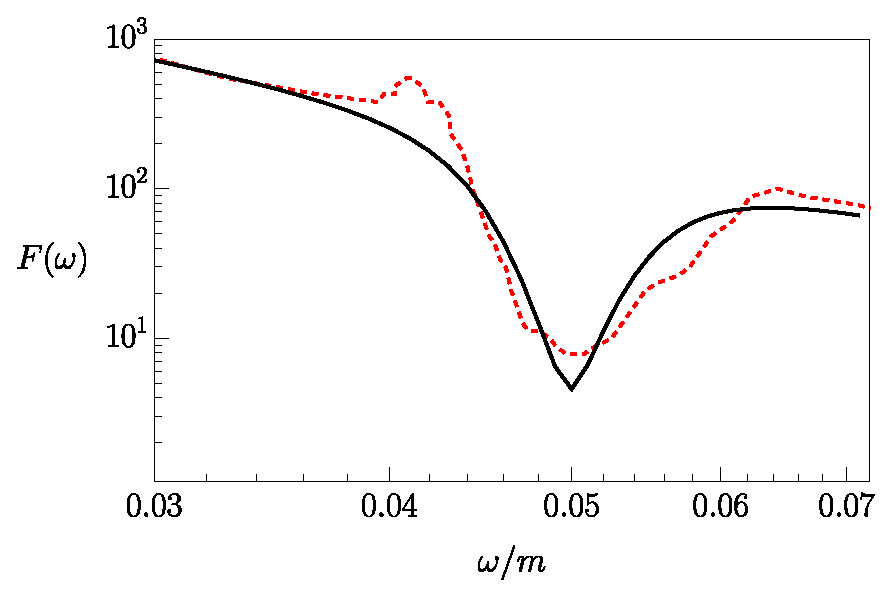
\includegraphics[width=\columnwidth]{fig1.eps}
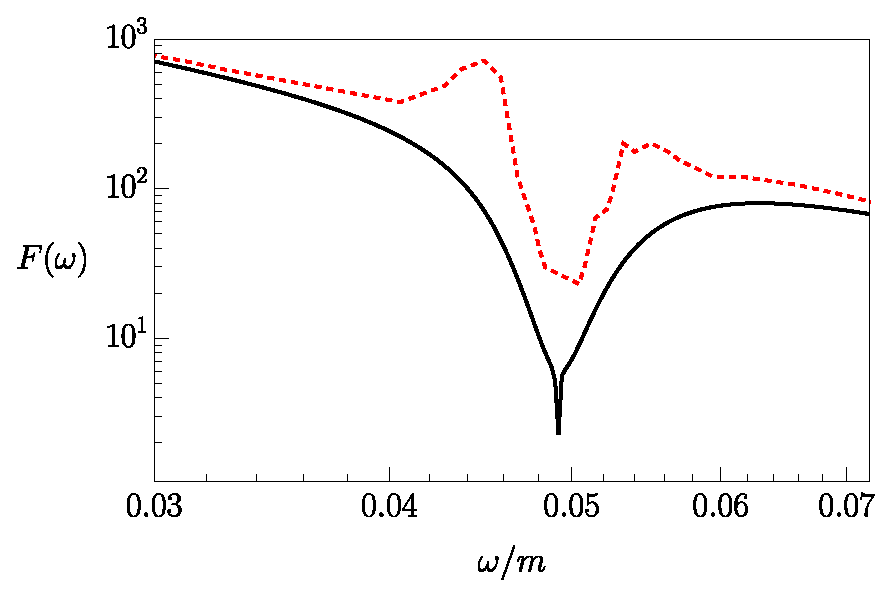
\includegraphics[width=\columnwidth]{fig2.eps}
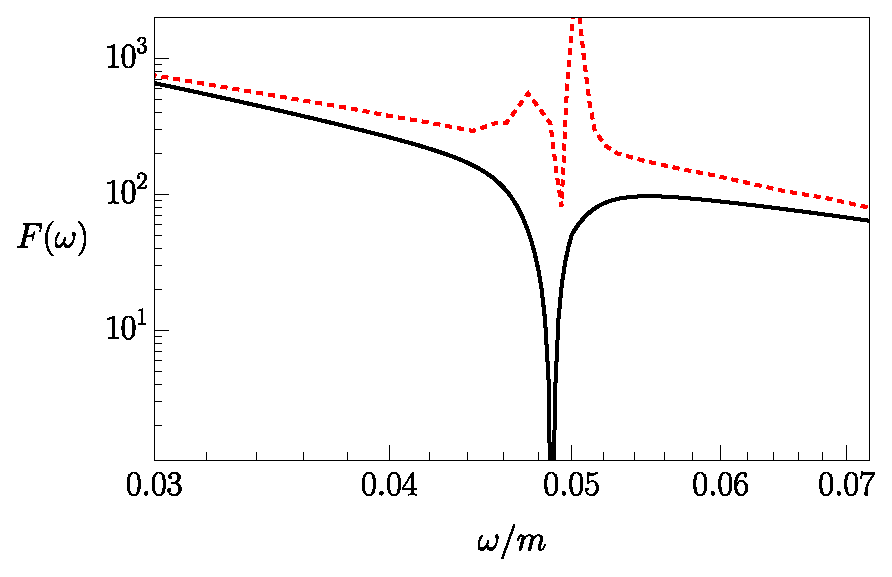
\includegraphics[width=\columnwidth]{fig3.eps}
\caption{Модель спектра фотона, усредненного по угловым~диапазонам (сверху вниз) \linebreak $\cos \theta\in [0.875, 1),[0.5, 0.625),(0, 0.125)$, а также по поляризации начального электрона при значениях параметров $B=0.05 B_e$, $T=3$ кэВ, $n_e=10^{19}$ см$^{-3}$, $z_{\mathrm{max}} = 1.5 \times 10^4$ см. Штриховая линия -- результаты работы Шенгерр и др., 2007 для поперечной оптической толщи $\tau_\perp^T=3 \times 10^{-4}$, что соответствует радиусу колонки $R=45$ см.}
\label{fig1}
\end{figure}
%%%%%%%%%%%%%%%%%%%%%%%%%%%%%%%%%%%%%%%%%%%%%%%%%%%%%%%%%

\section{Заключение}
\label{sect:concl}

Рассмотрено решение кинетического уравнения для нахождения функции распределения фотонов двух возможных поляризаций в равновесной нерелятивистской плазме электронов в относительно слабом магнитном поле $B\lesssim 10^{13}$ Гс с учетом резонанса на виртуальном электроне. Используя преобразование Лапласа и разложение функции распределения по полиномам Лежандра, мы свели задачу к решению системы дифференциальных уравнений на определение коэффициентов этого разложения. Решение представлено в виде интеграла в комплексной плоскости. Для значения магнитного поля $B\simeq10^{12}$ Гс и $T\simeq3$ кэВ в пределе малой оптической толщи был проведен сравнительный анализ модификации функции распределения фотона за счет резонансного комптоновского процесса с результатами работы (Шенгерр и др., 2007), полученными методом моделирования Монте-Карло. Показано, что полученное в данной работе аналитическое решение~(\ref{Solution}) хорошо согласуется с ними в области первого циклотронного резонанса.
 
Полученные результаты могут быть использованы для построения спектра излучения аккреционной колонки электронной плазмы. Для этого, согласно работе (Нисимура, 2008), можно разделить аккреционную колонку на малые области с постоянным значением магнитного поля и температуры, а результирующий спектр может быть найден как сумма резонансных вкладов от этих областей.


%%% Список литературы предваряется командой \begin{references}, а завершается командой \end{references}.
%%% Библиографическое описание каждой ссылки должно предваряться командой \reference
%%% и должно соответствовать Правилам для авторов Писем в Астрономический журнал.
%%% Список литературы должен быть упорядочен по алфавиту.
%%% Для сокращенных наименований часто цитируемых журналов можно использовать команды:
%%% \aap - Astron. Astrophys.
%%% \aapr - Astron. Astrophys. Rev.
%%% \aaps - Astron. Astrophys. Suppl. Ser.
%%% \aj - Astron. J.
%%% \ao - Appl. Optics
%%% \apj - Astrophys. J.
%%% \apjl - Astrophys. J.
%%% \apjs - Astrophys. J. Suppl. Ser.
%%% \apss - Astrophys. Space Sci.
%%% \araa - Ann. Rev. Astron. Astrophys.
%%% \asr - Adv. Space Res.
%%% \astl - Astron. Lett.
%%% \atel - Astron. Telegram
%%% \azh - Астрон. журн.
%%% \baas - BAAS       
%%% \iauc - IAU Circ.
%%% \jrasc - JRASC     
%%% \memras - MmRAS
%%% \mnras - Mon. Not. Roy. Astron. Soc.
%%% \nat{%%% \hbox{Nature
%%% \pra - Phys. Rev. A
%%% \prb - Phys. Rev. B
%%% \prc - Phys. Rev. C
%%% \prd - Phys. Rev. D
%%% \prl - Phys. Rev. Lett.    
%%% \pasp - Publ. Astron. Soc. Pacific
%%% \pasj - Publ. Astron. Soc. Japan
%%% \pazh - Письма в Астрон. журн.
%%% \qjras - QJRAS
%%% \skytel - S%%% \&T
%%% \solphys - Solar~Phys.
%%% \sovast - Sov.~Astron.
%%% \sval - Sov.~Astron. Lett.
%%% \ssr - Space~Sci. Rev.
%%% \zap - ZAp
\newpage
\begin{references}

\reference
Арайя и Хардинг (R.A. Araya and A.K. Harding) ``Cyclotron Line Features from Near-critical Magnetic Fields: The Effect of Optical Depth and Plasma Geometry'' Astrophys. J. {\bf 517}, 334 (1999).

\reference
Арайя и Хардинг (R.A. Araya-G\'ochez and A.K. Harding) ``Cyclotron Line Features from Near-Critical Fields. II. On the Effect of Anisotropic Radiation Fields'' Astrophys. J. {\bf 544}, 1067 (2000).

\reference
Беккер и Вольф (P.A. Becker and M.T. Wolff) ``Thermal and Bulk Comptonization in Accretion-powered X-ray Pulsars'' Astrophys. J. {\bf 654}, 435 (2007).

\reference 
Беккер и др. (P. A. Becker, D. Klochkov, G. Sch\"onherr et al.) ``Spectral formation in accreting X-ray pulsars: bimodal variation of the cyclotron energy with luminosity'' Astron. Astrophys. {\bf 544}, A123 (2012).

\reference
Беккер и Вольф (P.A. Becker and M.T. Wolff) ``A Generalized Analytical Model for Thermal and Bulk Comptonization in Accretion-powered X-Ray Pulsars'' Astrophys. J. {\bf 939}, 67 (2022).

\reference
Гинзбург В. Л., {\it Распространение электромагнитных волн в плазме} – 2-е изд., перераб. и доп. (М : Наука, 1967).

\reference
Компанеец А.С. ``Об установлении теплового равновесия между квантами и электронами'' ЖЭТФ {\bf 31}, 876 (1956) [A.S. Kompaneets ``The Settlement of Thermal Equilibrium in an Electron Gas Interactions with Radiation'' JETP {\bf 4} 730 (1957)].

\reference
Латал (H.G. Latal) ``Compton scattering in strong magnetic fields'' Astrophys. J. {\bf 309}, 372 (1986).

\reference
Любарский Ю.Э. ``Комптонизация в сверхсильном магнитном поле. I'' Астрофизика {\bf 28}, 183 (1988) [Yu. \'E. Lyubarskii ``Comptonization in a superstrong magnetic field. I'' Astrophys. {\bf 28} 106 (1988)].

\reference
Месарош и Нагель (P. M\'esz\'aros and W. Nagel) ``X-ray pulsar models. II. Comptonized spectra and pulse shapes'' Astrophys. J. {\bf 299}, 138 (1985).

\reference
Михалас (D. Mihalas), {\it Stellar Atmospheres} (San Francisco: W.H. Freeman \& Co., 1978).

\reference
Муштуков и др. (A.A. Mushtukov, V.F. Suleimanov, S.S. Tsygankov, and S. Portegies Zwart) ``Spectrum formation in X-ray pulsars at very low mass accretion rate: Monte-Carlo approach'' Mon. Not. R. Astron. Soc. {\bf 503}, 5193 (2021).

\reference
Муштуков и др. (A.A. Mushtukov, I.D. Markozov, V.F. Suleimanov et al.) ``Statistical features of multiple Compton scattering in a strong magnetic field'' Phys. Rev.~D {\bf 105}, 103027 (2022).

\reference
Муштуков и Портегис Цварт (A.A. Mushtukov and S. Portegies Zwart) ``Bright X-ray pulsars: how outflows influence beaming, pulsations and pulse phase lags'' Mon. Not. R. Astron. Soc. {\bf 518}, 5457 (2023).

\reference
Нисимура (O. Nishimura) ``The Influence of a Dipole Magnetic Field on the Structures of Cyclotron Lines'' Publ. Astron. Soc. Jpn. {\bf 55}, 451 (2003).

\reference
Нисимура (O. Nishimura) ``Cyclotron Lines Formed in an Infalling Plasma Slab on a Neutron Star Surface'' Publ. Astron. Soc. Jpn. {\bf 57}, 769 (2005).

\reference
Нисимура (O. Nishimura) ``Superposition of Cyclotron Lines Emerging from Local Regions on a Neutron Star Surface'' Astrophys. J. {\bf 672}, 1127 (2008).

\reference
Нисимура (O. Nishimura) ``Variations of Cyclotron Line Energy with Luminosity in Accreting X-Ray Pulsars'' Astrophys. J. {\bf 730}, 106 (2011).

\reference
Потехин и др. (A.Y. Potekhin, D. Lai, G. Chabrier, and W.C.G. Ho), ``Electromagnetic polarization in partially ionized plasmas with strong magnetic fields and neutron star atmosphere models'' Astrophys. J. {\bf 612}, 1034 (2004)

\reference
Румянцев и др. (D.A. Rumyantsev, M.V. Chistyakov, T.A. Puhov) ``Resonant Compton Scattering in a Magnetized Medium'' Phys. At. Nucl. {\bf 89}, 234 (2026а).

\reference
Румянцев и др. (Румянцев Д.А., Шленев Д.М., Ярков А.А.) ``Резонансное комптоновское рассеяние в замагниченной среде''  ЖЭТФ {\bf 169}, 607 (2026б).

\reference
Чистяков и др. (M.V. Chistyakov, D.A. Rumyantsev, N.S. Stus') ``Photon splitting in a strongly magnetized plasma'' Phys. Rev.~D {\bf 86}, 043007 (2012).

\reference
Шабад А.Е. Тр. ФИАН СССР “Поляризационные эффекты во внешних калибровочных полях” {\bf 192}, 5 (1988).

\reference
Шенгерр (G. Sch\"onherr, J. Wilms, P. Kretschmar et al.) ``A model for cyclotron resonance scattering features'' Astron. Astrophys. \({\bf 472}, 353 (2007).\)

\reference 
Ярков и Румянцев (A.A. Yarkov and D.A. Rumyantsev) ``Resonant Compton Scattering of Photons by Electrons in a Strong Magnetic Field'' Phys. At. Nucl. {\bf 80}, 890 (2023).


\end{references}

\end{document}